\documentclass{article}
\usepackage{graphicx}
\usepackage[margin=1.5cm]{geometry}
\usepackage{amsmath}

\begin{document}
\twocolumn

\title{Monday Warm Up: Unit 2, DC Circuits}
\author{Prof. Jordan C. Hanson}

\maketitle

\section{Memory Bank}

\begin{itemize}
\item $V = IR$ ... The macroscopic version of Ohm's law
\item $R_{\rm tot} = R_1 + R_2$ ... Resistors in series.
\item $R_{\rm tot}^{-1} = R_1^{-1} + R_2^{-1}$ ... Resistors in parallel.
\item $V_{\rm terminal} = \mathcal{E} - Ir$ ... The terminal voltage on a battery with emf $\mathcal{E}$, current $I$, and \textit{internal resistance} $r$.
\item $P = IV = I^2 R = V^2/R$ ... Expressions for the power in a DC circuit.
\item $(R_1 \pm \sigma_1) + (R_2 \pm \sigma_2) = (R_1 + R_2) \pm \sqrt{\sigma_1^2 + \sigma_2^2}$ Adding two measurements with associated errors.
\end{itemize}

\begin{figure}
\centering
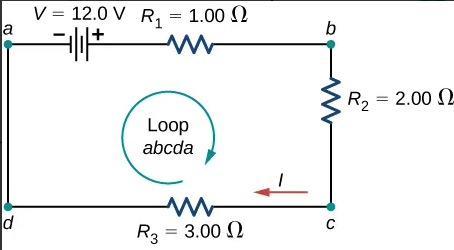
\includegraphics[width=0.35\textwidth,trim=0.1cm 0cm 0cm 0.1cm,clip=true]{figures/kirchhoff_1.png}
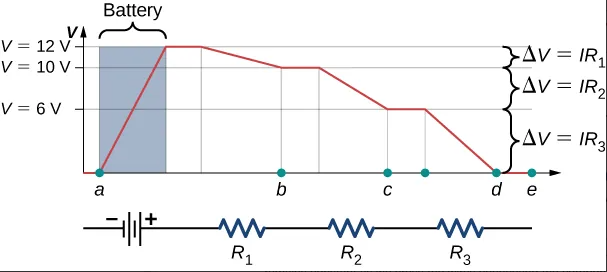
\includegraphics[width=0.35\textwidth,trim=0cm 0.1cm 0.1cm 0cm,clip=true]{figures/kirchhoff_2.png}
\caption{\label{fig:1} (Top) Three resistors in series with a battery emf. (Bottom) Chart of the voltage as a function of location around the series loop.}
\end{figure}

\section{Kirchhoff's Rules}

\begin{enumerate}
\item Consider Fig. \ref{fig:1} (top).  (a) What current flows from the battery? (b) What is the total power consumption? \\ \vspace{1.5cm}
\item Consider  Fig. \ref{fig:1} (bottom).  Imagine moving along the path from point \textit{a} to point \textit{d}, and then back to \textit{a.}  According to the chart in Fig. \ref{fig:1} (bottom), what is the total change in voltage? \\ \vspace{2cm}
\item The loop technique in the previous exercise technically works for any loop within a circuit (conservation of energy).  Consider Fig. \ref{fig:2}, and let $I_3$ be the current through $R_3$, $I_4$ be the current through $R_4$, and $I_1$ be the current through $R_1$.  (a) Use the loop technique to prove that
\begin{equation}
V_1 - I_3 R_3 - I_1 R_2 - I_1 R_1 = 0
\end{equation}
(b) Use a loop involving $V_2$ to create a similar equation as found in part (a) for the lower loop. \\ \vspace{2cm}
\item The \textit{junction technique} states that (by charge conservation) the currents leaving a junction should sum to the currents entering a junction.  Using the loop and the junction techniques, solve for all currents through all resistors in Fig. \ref{fig:2}.
\end{enumerate}

\begin{figure}
\centering
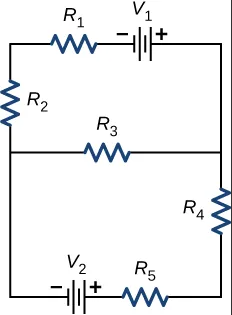
\includegraphics[width=0.175\textwidth,trim=0cm 0cm 0.1cm 0.0cm,clip=true]{figures/kirchhoff_3.png}\caption{\label{fig:2} A circuit with two batteries and five resistors.}
\end{figure}

\end{document}
